%!TEX TS-program = xelatex
%!TEX encoding = UTF-8 Unicode

\documentclass[a4paper]{article}

\usepackage{xltxtra}
\usepackage{amsfonts}
\usepackage{polyglossia}
\usepackage{fancyhdr}
\usepackage{geometry}
\usepackage{dsfont}
\usepackage{amsmath}
\usepackage{amsthm}
\usepackage{physics}
\usepackage{float}
\usepackage{tikz}
\usepackage{bm}
\usepackage[shortlabels]{enumitem}
\usetikzlibrary{shapes,arrows,positioning}

\geometry{a4paper,left=15mm,right=15mm,top=20mm,bottom=20mm}
\pagestyle{fancy}
\lhead{Devon Morris}
\chead{Detection \& Estimation Theory - Homework 2}
\rhead{\today}
\cfoot{\thepage}

\setlength{\headheight}{23pt}
\setlength{\parindent}{0.0in}
\setlength{\parskip}{0.0in}

\newtheorem{prop}{Proposition}
\newtheorem*{sol}{Solution}

\tikzset{
block/.style = {draw, fill=white, rectangle, minimum height=3em, minimum width=3em},
tmp/.style  = {coordinate}, 
sum/.style= {draw, fill=white, circle, node distance=1cm},
input/.style = {coordinate},
output/.style= {coordinate},
pinstyle/.style = {pin edge={to-,thin,black}
}
}

\begin{document}

\section*{Problem 1}%
What is the characteristic function for a general bivariate normal?

\subsection*{Solution}%
According to the 2.150 in the book, we have that for two normally distributed random variables $X_1 \sim \mathcal{N}(m_1, \sigma_1^2)$, $X_2 \sim \mathcal{N}(m_2, \sigma_2^2)$ with covariance, $\sigma_{12}$, that the characteristic function is
\[
  \begin{aligned}
    \phi(\omega_1, \omega_2) &= \text{exp} \left( -\frac{1}{2}\left( [\omega_1, \omega_2]R \begin{bmatrix}
      \omega_1 \\
      \omega_2
\end{bmatrix} -j2[\omega_1, \omega_2]
  \begin{bmatrix}
    m_1 \\
    m_2
  \end{bmatrix}\right)\right) \\
                             &=  \text{exp} \left( -\frac{1}{2}\left( \sigma_1^2\omega_1^2 + \sigma_2^2\omega_2^2 + 2\sigma_{12}\omega_1\omega_2 - j2(\omega_1m_1 + \omega_2m_2) \right)  \right)
  \end{aligned}
\]

\section*{Problem 2}%
Let $(U_1, U_2)$ denote independent normal random variables with respective means of zero and respective variances of $(\sigma_1^2, \sigma_2^2)$. Define $(X_1, X_2)$ as the following rotation of $(U_1,U_2)$:

\[
  \begin{bmatrix}
    X_1 \\
    X_2
  \end{bmatrix}
  = 
  \begin{bmatrix}
    \cos \theta & -\sin \theta \\
    \sin \theta & \cos \theta
  \end{bmatrix}
  \begin{bmatrix}
    U_1 \\
    U_2
  \end{bmatrix}
\]
Draw the contours of constant probability for $(X_1, X_2)$ and compare those of $(U_1, U_2)$.

\subsection*{Solution}%
We first note that the covariance matrix of $U_1$ and $U_2$ is just 
\[
  \begin{bmatrix}
    \sigma_1^2 & 0 \\
    0 & \sigma_2^2 
  \end{bmatrix}
\]
Let $X = [X_1, X_2]^\top$. We have that $E[X] = [0, 0]^\top$, and our covariance matrix is
\[
  \begin{aligned}
    E[XX^\top] &= E \left[
  \begin{bmatrix}
    \cos \theta & -\sin \theta \\
    \sin \theta & \cos \theta
  \end{bmatrix}
  UU^\top
  \begin{bmatrix}
    \cos \theta & \sin \theta \\
    -\sin \theta & \cos \theta
\end{bmatrix} \right]\\
               &=
  \begin{bmatrix}
    \cos \theta & -\sin \theta \\
    \sin \theta & \cos \theta
  \end{bmatrix}
  E[UU^\top]
  \begin{bmatrix}
    \cos \theta & \sin \theta \\
    -\sin \theta & \cos \theta
  \end{bmatrix} \\
               &= \begin{bmatrix}
    \cos \theta & -\sin \theta \\
    \sin \theta & \cos \theta
  \end{bmatrix}
  \begin{bmatrix}
    \sigma_1^2 & 0 \\
    0 & \sigma_2^2 
  \end{bmatrix}
  \begin{bmatrix}
    \cos \theta & \sin \theta \\
    -\sin \theta & \cos \theta
  \end{bmatrix}
  \end{aligned}
\]
These are plotted with the values $\sigma_1^2 = 1$ and $\sigma_2^2=2$ and $\theta = \pi/4$. Basically, you just get a rotation of the contours of constant probability.

\begin{figure}[H]
\begin{center}
  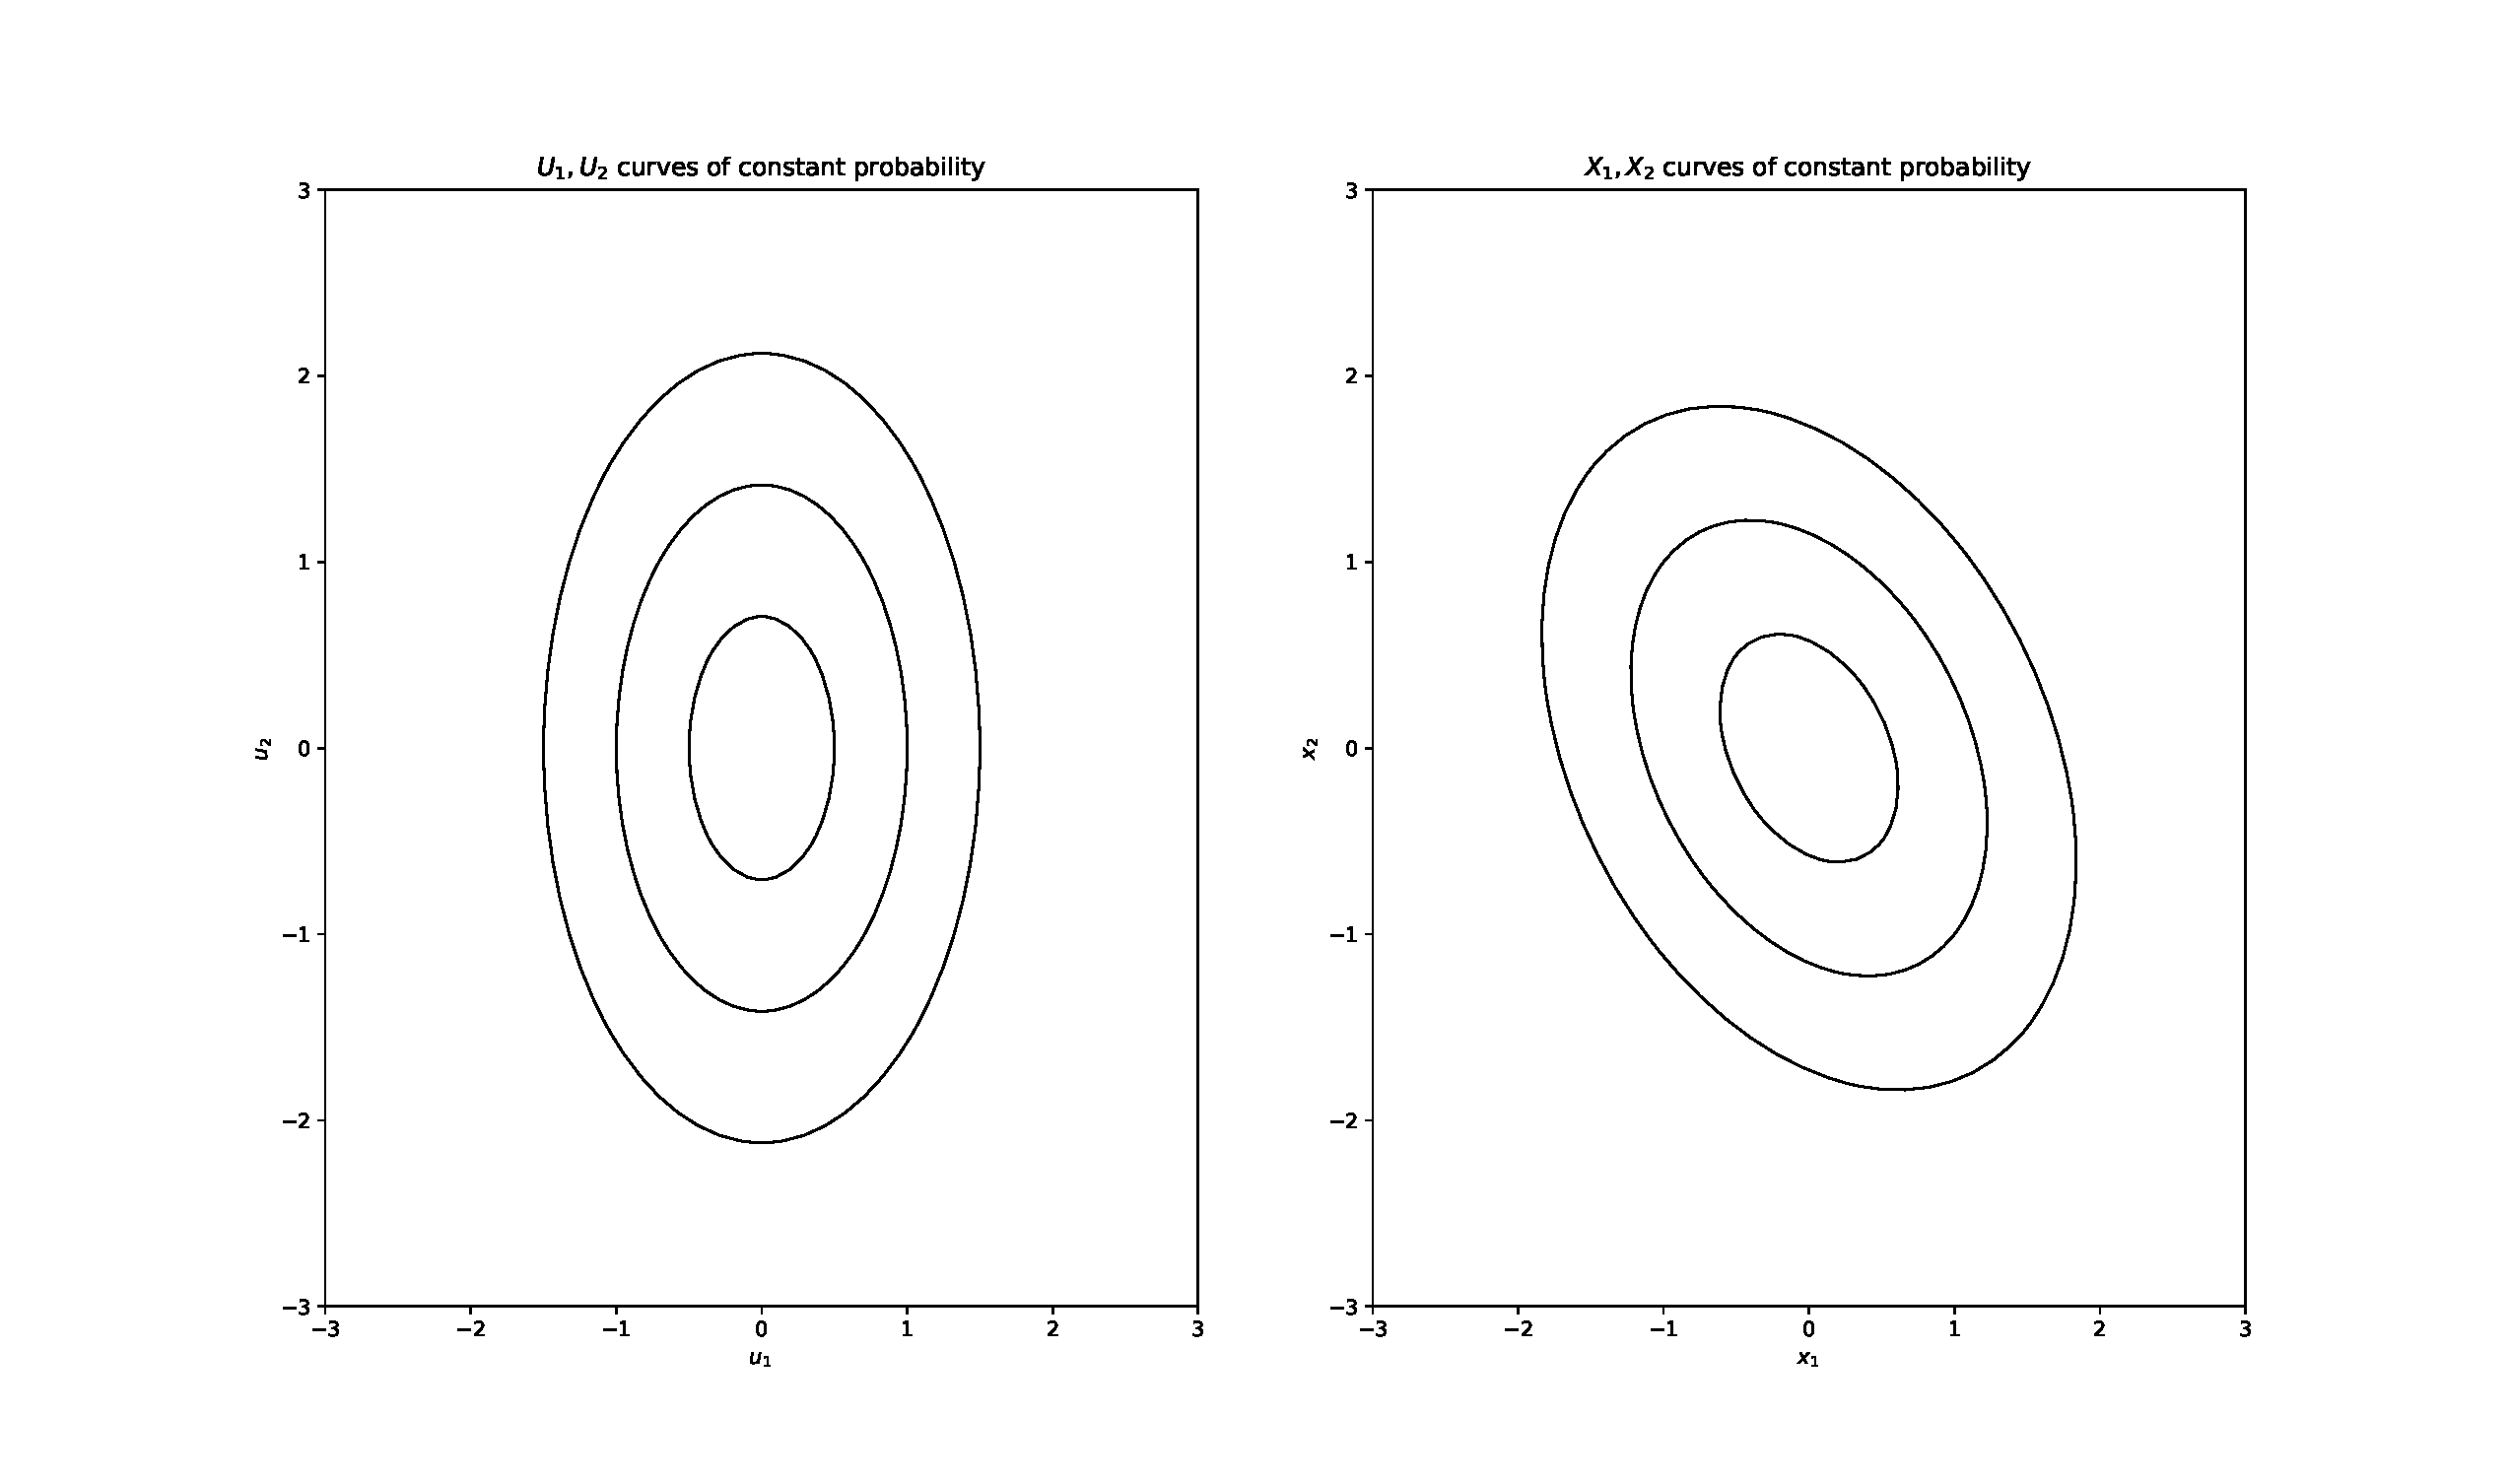
\includegraphics[scale=0.4]{hw2-2.eps}
\end{center}
\caption{curves of constant probability}
\label{fig:Curves of Constant probability}
\end{figure}

\section*{Problem 3}%
Let $X = [X_1, X_2]^\top$ denote a bivariate normal random vector. Assume 
\[
  E[X] = 0 \quad \text{and} \quad E[XX^\top] = 
  \begin{bmatrix}
    1 & \rho \\
    \rho & 1
  \end{bmatrix}
\]

Define $Y_1 = X_1 + X_2$ and $Y_2 = -X_1 + X_2$.
\begin{enumerate}[a.]
  \item Find the joint distributions of $Y_1$ and $Y_2$; find the marginal distributions of $Y_1$ and $Y_2$.
  \item Find the conditional density of $X_1$, given $Y_1$; find the conditional density of $X_1$, given $Y_2$.
  \item Find the conditional mean and variance of $X_1$, given $Y_1$; find the conditional mean and variance of $X_1$, given $Y_2$.
\end{enumerate}

\subsection*{Solution}%

\subsubsection*{Part a}%

We first note that 
\[
  \begin{bmatrix}
    Y_1 \\
    Y_2
  \end{bmatrix}
  =
  \begin{bmatrix}
    1 & 1 \\
    -1 & 1
  \end{bmatrix}
  \begin{bmatrix}
    X_1 \\
    X_2
  \end{bmatrix}
\]
Since this is a linear transformation of a zero-mean bivariate random normal vector we have a zero-mean bivariate random normal vector with covariance
\[
  \begin{aligned}
  E \left[ YY^\top \right] &= 
  \begin{bmatrix}
    1 & 1 \\
    -1 & 1
  \end{bmatrix}
  \begin{bmatrix}
    1 & \rho \\
    \rho & 1
  \end{bmatrix}
  \begin{bmatrix}
    1 & -1 \\
    1 & 1
  \end{bmatrix} \\
                           &=
   \begin{bmatrix}
     1 + \rho & 1 + \rho \\
     -1 + \rho & 1 - \rho
   \end{bmatrix}
  \begin{bmatrix}
    1 & -1 \\
    1 & 1
  \end{bmatrix} \\
                           &=
   \begin{bmatrix}
     2(1 + \rho) & 0 \\
     0 & 2(1 - \rho)
   \end{bmatrix}
  \end{aligned}
\]
At this point we can write down the joint density
\[
  \begin{aligned}
    f_{Y_1,Y_2}(y_1, y_2) &=  \frac{1}{(2\pi)^{2/2} (2(1+\rho))^{1/2}(2(1-\rho))^{1/2}} \text{exp} \left(-\frac{1}{2} \left( \frac{y_1^2}{2(1+\rho)} + \frac{y_2^2}{2(1-\rho)} \right)  \right)
  \end{aligned}
\]
However, we can factor this in a nice way, specifically
\[
  \begin{aligned}
    f_{Y_1,Y_2}(y_1, y_2) &=  \frac{1}{(2\pi)^{2/2} (2(1+\rho))^{1/2}(2(1-\rho))^{1/2}} \text{exp} \left(-\frac{1}{2} \left( \frac{y_1^2}{2(1+\rho)} + \frac{y_2^2}{2(1-\rho)} \right)  \right) \\
                          &= \frac{1}{(2\pi)^{1/2} (2(1+\rho))^{1/2}} \text{exp}\left(-\frac{y_1^2}{4(1 + \rho)}\right) \frac{1}{(2\pi)^{1/2} (2(1-\rho))^{1/2}} \text{exp}\left(-\frac{y_2^2}{4(1 - \rho)}\right) 
  \end{aligned}
\]
From this, we can see that $Y_1$ and $Y_2$ are independent and the marginal distributions are
\[
  \begin{aligned}
    f_{Y_1}(y_1) &= \frac{1}{(2\pi)^{1/2} (2(1+\rho))^{1/2}} \text{exp}\left(-\frac{y_1^2}{4(1 + \rho)}\right) \\
    f_{Y_2}(y_2) &= \frac{1}{(2\pi)^{1/2} (2(1-\rho))^{1/2}} \text{exp}\left(-\frac{y_2^2}{4(1 - \rho)}\right) 
  \end{aligned}
\]

\subsubsection*{Part b}%
Note that 
\[
  F_{X_1|Y_1}(x_1|y_1) = P[X_1 \leq x_1 | Y_1 = y_1] = P[Y_1 - X_2 \leq x_1 | Y_1 = y_1] = P[X_2 \geq y_1 - x_1] = 1 - F_{X_2}(y_1 - x_1)
\]
Differentiating, we have that
\[
  \begin{aligned}
    f_{X_1|Y_1}(x_1|y_1) &= \dv{}{x_1} \left(1 - F_{X_2}(y_1 - x_1) \right)\\
                         &= f_{X_2}(y_1 - x_1) \\
                         &= \frac{1}{(2\pi)^{n/2}} \text{exp} \left( -\frac{(y_1-x_1)^2}{2} \right)\\
                         &= \frac{1}{(2\pi)^{n/2}} \text{exp} \left( -\frac{(x_1-y_1)^2}{2} \right)
  \end{aligned}
\]

Similarly,
\[
  F_{X_1|Y_2}(x_1|y_2) = P[X_1 \leq x_1 | Y_2 = y_2] = P[Y_2 + X_2 \leq x_1 | Y_2 = y_2] = P[X_2 \leq x_1 - y_2] = F_{X_2}(x_1 - y_2)
\]
Differentiating, we have
\[
  \begin{aligned}
  f_{X_1|Y_2}(x_1|y_2) &= \dv{}{x_1} \left(F_{X_2}(x_1 - y_2)\right)\\
                       &= f_{X_2}(x_1 - y_2) \\
                       &= \frac{1}{(2\pi)^{n/2}} \text{exp} \left( -\frac{(x_1-y_2)^2}{2} \right)
  \end{aligned}
\]

\subsubsection*{Part c}%
Since we saw in part b that $X_1|Y_1$ and $X_1|Y_2$ are normally distributed, we have that
\[
  E[X_1|Y_1] = 0 \quad \text{and} \quad \text{Var}[X_1|Y_1] = 1
\]
and
\[
  E[X_1|Y_2] = 0 \quad \text{and} \quad \text{Var}[X_1|Y_2] = 1
\]
simply from looking at their densities.

\section*{Problem 4}%
Begin with $X \sim \mathcal{N}(0, U\Lambda^2 U^\top)$ with $U$ orthogonal and $\Lambda^2$ diagonal. Define $Y = \Gamma U^\top X$. Choose $\Gamma$ to make $Y^\top Y$ chi-squared distributed with $r$ degrees of freedom.

\subsection*{Solution}%
Note that $\Lambda^2$ can be factored as
\[
  \Lambda^2 = 
  \begin{bmatrix}
    \lambda_1^2 & 0 & \cdots & 0 \\
    0 & \lambda_2^2 &\cdots & 0 \\
    \vdots & \vdots & \ddots & \vdots \\
    0 & 0 & \cdots & \lambda_n^r
  \end{bmatrix}
  =
  \begin{bmatrix}
    \lambda_1 & 0 & \cdots & 0 \\
    0 & \lambda_2 &\cdots & 0 \\
    \vdots & \vdots & \ddots & \vdots \\
    0 & 0 & \cdots & \lambda_r
  \end{bmatrix}^2
\]
Where the $\lambda_i$ are the square roots of $\lambda_i^2$. Let 
\[
  \Gamma = 
  \begin{bmatrix}
    1/\lambda_1 & 0 & \cdots & 0 \\
    0 & 1/\lambda_2 &\cdots & 0 \\
    \vdots & \vdots & \ddots & \vdots \\
    0 & 0 & \cdots & 1/\lambda_r
  \end{bmatrix}
\]
So note that we have $E[Y] = 0$, since $X$ was zero mean. and 
\[
  \begin{aligned}
    \text{Var}(Y) &= E[YY^\top] = E[\Gamma U^\top XX^\top U \Gamma^\top] \\
                  &= \Gamma U^\top U \Lambda^2 U^\top U \Gamma^\top \\
                  &= \Gamma \Lambda^2 \Gamma^\top \\
                  &= I
  \end{aligned}
\]
So we have that $Y$ is a vector of independent standard normal random variables. Note that
\[
Y^\top Y = Y_1^2 + Y_2^2 + \cdots + Y_r^2
\]
since, each $Y_i$ is standard normal, then $Y^\top Y$ is chi-squared distributed with $r$ degrees of freedom.

\section*{Problem 5}%
Prove $E[Q] = \text{tr}(PR)$ and $\text{Var}[Q] = 2 \text{tr} ((PR)^2)$ when $Q = (X - m)^\top P (X-m)$ and $X \sim \mathcal{N}(m, R)$.

\subsection*{Solution}%
Since the trace of a scalar is just itself and trace is linear. 
\[
  \begin{aligned}
    E[Q] &= E \left[ (X-m)^\top P (X-m) \right] \\
         &= \text{tr} \left(E \left[ (X-m)^\top P (X-m) \right] \right) \\
         &= E \left[ \text{tr}\left((X-m)^\top P (X-m)\right)\right]
  \end{aligned}
\]
Now using the cyclic property of the trace, we have
\[
  \begin{aligned}
    E[Q] &= E \left[ \text{tr}\left((X-m)^\top P (X-m)\right)\right] \\
         &= E \left[ \text{tr}\left(P (X-m)(X-m)^\top\right)\right] \\
         &= \text{tr}\left(P E[(X-m)(X-m)^\top]\right) \\
         &= \text{tr}\left(P E[(X-m)(X-m)^\top]\right) \\
         &= \text{tr} \left( PR \right)
  \end{aligned}
\]
To find the variance we will use the characteristic function of $Q$
\[
  \phi(\omega) = \frac{1}{\text{det}\left( I + 2j\omega PR \right)^{1/2}}
\]
We have that
\[
  \begin{aligned}
  E[Q^2] = -\eval{\dv[2]{}{\omega}}_{\omega=0} \phi(\omega) \\
  \end{aligned}
\]
Performing the first derivative we have
\[
  \dv{}{\omega} \phi(\omega) = - \frac{1}{2\text{det}(I + 2j\omega PR)^{1/2}} \text{tr}( (I+2j\omega PR)^{-1} 2jPR)
\]
The second derivative gives us
\[
  \begin{aligned}
    \dv[2]{}{\omega} \phi(\omega) &=
  \frac{1}{4\text{det}(I + 2j\omega PR)^{1/2}} \text{tr}((I+2j\omega PR)^{-1} 2jPR)^2  \\
                                  &-\frac{1}{2\text{det}\left( I + 2j\omega PR \right)^{1/2}}\text{tr} \left(-(I+2j\omega PR)^{-1}2jPR(I + 2j\omega PR)^{-1} 2jPR \right)
  \end{aligned}
\]
Evaluating this derivative at 0, we get
\[
  - \eval{\dv[2]{}{\omega}}_{\omega = 0} \phi(\omega) =  -\frac{(2j)^2}{4} \text{tr}((PR))^2 - \frac{(2j)^2}{2} \text{tr}((PR)^2) = \text{tr}((PR))^2 + 2 \text{tr}((PR)^2)
\]
Which is the second moment of $Q$. We finally have that
\[
  \text{Var}[Q] =  E[Q^2] - E[Q]^2 =  \text{tr}((PR))^2 + 2 \text{tr}((PR)^2) - \text{tr}((PR))^2 = 2 \text{tr}((PR)^2)
\]

\end{document}

